%%%%%%%%%%%%%%%%%%%%%%%%%%%%%%%%%%%%%%%%%%%%%%%%%%%%%%%%%%%%%%%%%%%%%%
% CS637: Database-Backed Websites
% Copyright 2015 Pejman Ghorbanzade <mail@ghorbanzade.com>
% Creative Commons Attribution-ShareAlike 4.0 International License
% More info: https://bitbucket.org/ghorbanzade/umb-cs637-2015s
%%%%%%%%%%%%%%%%%%%%%%%%%%%%%%%%%%%%%%%%%%%%%%%%%%%%%%%%%%%%%%%%%%%%%%

\section*{Question 5}

Consider the HTML of the \href{http://topcat.cs.umb.edu/book_apps/ch05_guitar_shop/product_manager/product_list.php}{\texttt{product\_list.php}} web page. Simplify it to plain HTML, that is, drop all the PHP and fill in data on the categories and two products right in the HTML. You don't need to change the CSS for this. Show the HTML in your paper. You can continue to include the header and footer files.

\subsection*{Solution}

The pure HTML code generating the web page is given below.

\begin{lstlisting}
%\begin{minted}[fontsize=\small,tabsize=8,linenos, firstnumber=1,frame=lines,framerule=1pt]{html}
<!DOCTYPE html>
<html>
  <head>
    <title>My Guitar Shop</title>
    <link rel="stylesheet" type="text/css" href="/book_apps/ch05_guitar_shop/main.css">
  </head>
  <body>
    <header>
      <h1>My Guitar Shop</h1>
    </header>
    <main>
      <h1>Product List</h1>
      <aside>
        <h2>Categories</h2>
        <nav>
        <ul>
          <li><a href="?category_id=1">Guitars</a></li>
          <li><a href="?category_id=2">Basses</a></li>
          <li><a href="?category_id=3">Drums</a></li>
        </ul>
        </nav>
      </aside>
      <section>
        <h2>Drums</h2>
        <table>
          <tr>
            <th>Code</th>
            <th>Name</th>
            <th class="right">Price</th>
            <th>&nbsp;</th>
          </tr>
          <tr>
            <td>ludwig</td>
            <td>Ludwig 5-Piece Drum Set with Cymbals</td>
            <td class="right">699.99</td>
            <td>
            <form action="." method="post">
              <input type="hidden" name="action" value="delete_product">
              <input type="hidden" name="product_id" value="1">
              <input type="hidden" name="category_id" value="1">
              <input type="submit" value="Delete">
            </form>
            </td>
          </tr>
          <tr>
            <td>tama</td>
            <td>Tama 5-Piece Drum Set with Cymbals</td>
            <td class="right">799.99</td>
            <td>
              <form action="." method="post">
                <input type="hidden" name="action" value="delete_product">
                <input type="hidden" name="product_id" value="2">
                <input type="hidden" name="category_id" value="2">
                <input type="submit" value="Delete">
              </form>
            </td>
          </tr>
        </table>
        <p class="last_paragraph">
          <a href="?action=show_add_form">Add Product</a>
        </p>
      </section>
    </main>
    <footer>
      <p class="copyright">&copy; 2015 My Guitar Shop, Inc.</p>
    </footer>
  </body>
</html>
%\end{minted}
\end{lstlisting}

Using this code the front-end will look as depicted in Figure \ref{fig5}.

\begin{figure}[H]\centering
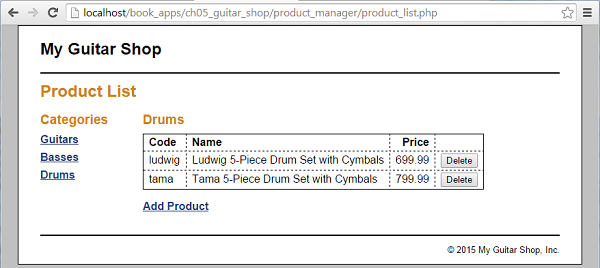
\includegraphics{\pngDirectory/hw02/hw02q05f05.png}
\caption{Reconstructed \texttt{product\_list.html} file}
\label{fig5}
\end{figure}

\end{document}
